\documentclass[25pt,a1paper]{tikzposter}
\geometry{paperwidth=80cm,paperheight=200cm}
%% Tikzposter is highly customizable: please see
%% https://bitbucket.org/surmann/tikzposter/downloads/styleguide.pdf

% a guide: https://roboticsconference.org/information/sample-poster2.pdf

%% Available themes: see also
%% https://bitbucket.org/surmann/tikzposter/downloads/themes.pdf
% \usetheme{Default}
% \usetheme{Rays}
 \usetheme{Basic}
% \usetheme{Simple}
%\usetheme{Envelope}
% \usetheme{Wave}
% \usetheme{Board}
% \usetheme{Autumn}
% \usetheme{Desert}

%% Further changes to the title etc is possible
% \usetitlestyle{Default}
% \usetitlestyle{Basic}
% \usetitlestyle{Empty}
% \usetitlestyle{Filled}
% \usetitlestyle{Envelope}
% \usetitlestyle{Wave}
% \usetitlestyle{verticalShading}

\usepackage{fontspec}
\setmainfont{FreeSerif}
\setsansfont{FreeSans}

\author{Taipei Medical University}
\title{HEALTH CARE BEYOND
BORDERS}
\institute{Taiwan Medical Mission in the Republic of Somaliland}
%% Optional title graphic
\titlegraphic{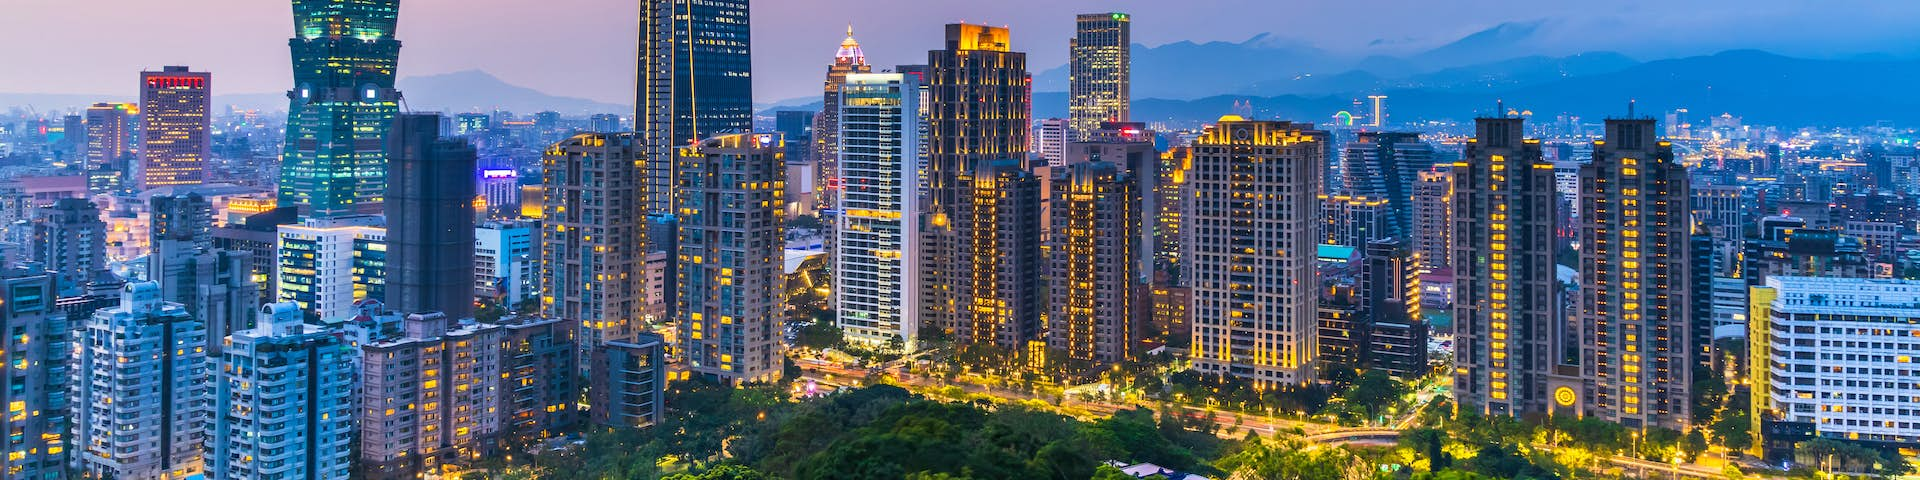
\includegraphics[width=0.7\linewidth]{Taipei_5f994223a0add.jpg}}
% 24cm
%% Uncomment to switch off tikzposter footer
% \tikzposterlatexaffectionproofoff

\begin{document}
\maketitle

\block{TMU Healthcare System}{
\begin{itemize}

With outstanding medical research and accomplishments, Taipei Medical University (TMU) has established itself as one of Asia's leading institutions for medical education. The Taipei Medical University Hospital (TMUH), WanFang Medical Center (TMWH), Shuang-Ho Hospital, TMU Taipei Cancer Center, Taipei Neuroscience Institute, and TMU LiHuiLi Hospital in Ningbo, China, are all part of the TMU Health System.
TMU Healthcare System is better able to help medical professionals and patients in Taiwan and around the world by combining the existing clinical resources with cloud resources in their Information and Communications Technology (ICT) in medicine.

\item \#TMUtw 
\item \#TaipeiMedicalUniversity 
\item \#CloudICT
\item \#Telemedicine
\item \#Bioinformatics
%\item we try to do that.
\end{itemize}
}

\note[rotate=8, connection, width = 6cm, targetoffsetx=-20cm, targetoffsety=-07cm
% roundedcorners=15, 
]{Mashallah\\ ما شاء الله}

\begin{columns}

\column{0.7}
\block{What does TMU are}{
\begin{itemize}
TMU Spotlight showcases impressive outcomes from our partnership collaboration, research excellence, talent development, and the University’s commitment to making a positive social impact.

%\item We try to do this. what?
%\item we try to do that.
\end{itemize}

\innerblock{TMU's Hospitals}{
% Figures of TMU
\begin{minipage}{0.45\linewidth}
  \centering
    \begin{tikzfigure}[]
    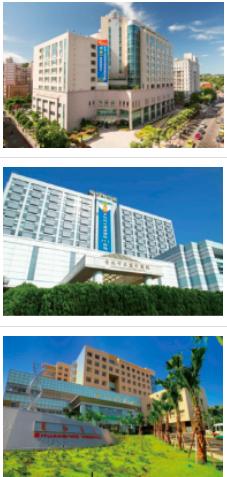
\includegraphics[width=0.8\linewidth]{TMU123.jpg}
%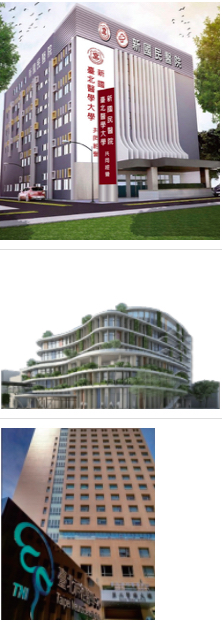
\includegraphics[width=0.5\linewidth]{TMU456.jpg}
    \end{tikzfigure}
\end{minipage}\hfill
\begin{minipage}{0.45\linewidth}
  \centering
%\innerblock{TMU's Hospitals}{
    \begin{tikzfigure}[]
    %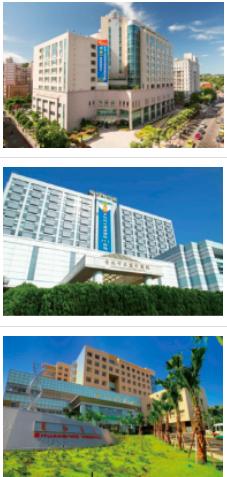
\includegraphics[width=0.5\linewidth]{TMU123.jpg}
    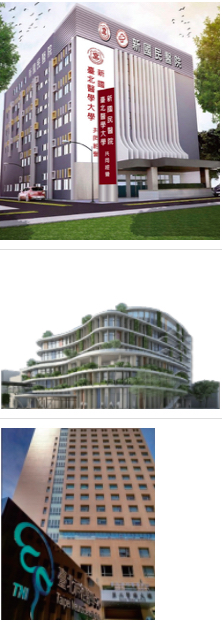
\includegraphics[width=0.6\linewidth]{TMU456.jpg}
    \end{tikzfigure}
\end{minipage}
} % end of innerblock

} % end of block

\column{0.3}
\block{What does TMU do}{
\begin{itemize}
\item To provide medical services based on special demand 
\item Clinical capacity building for health personnel individuals \item Public health research and improvements
\item Through \textbf{telemedicine} to provide international medical aid
\end{itemize}

% Taiwan Task Force For Medical Travel
\begin{tikzfigure}[Taiwan Task Force For Medical Travel]
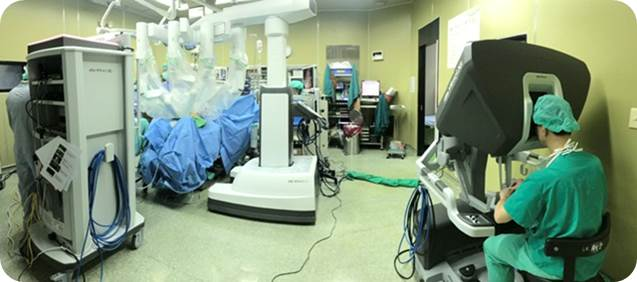
\includegraphics[width=\linewidth]{TMWH_daVinci.jpg}
\end{tikzfigure}

% thoracic surgery, otolaryngology, neurosurgery, general surgery, colorectal surgery, urology, obstetrics and gynecology, orthopedics
% http://www.taiwanhealthcare.com/product/40&path=60

Robotic arm assisted laparoscopic surgery (\textbf{Da Vinci system}) is minimal invasive surgery for
urology, obstetrics & gynecology, general surgery (thyroid, breast), colorectal surgery.
}

\end{columns}

%%
\block{Hybride Operation Theatre}{%
\begin{tikzfigure}[]
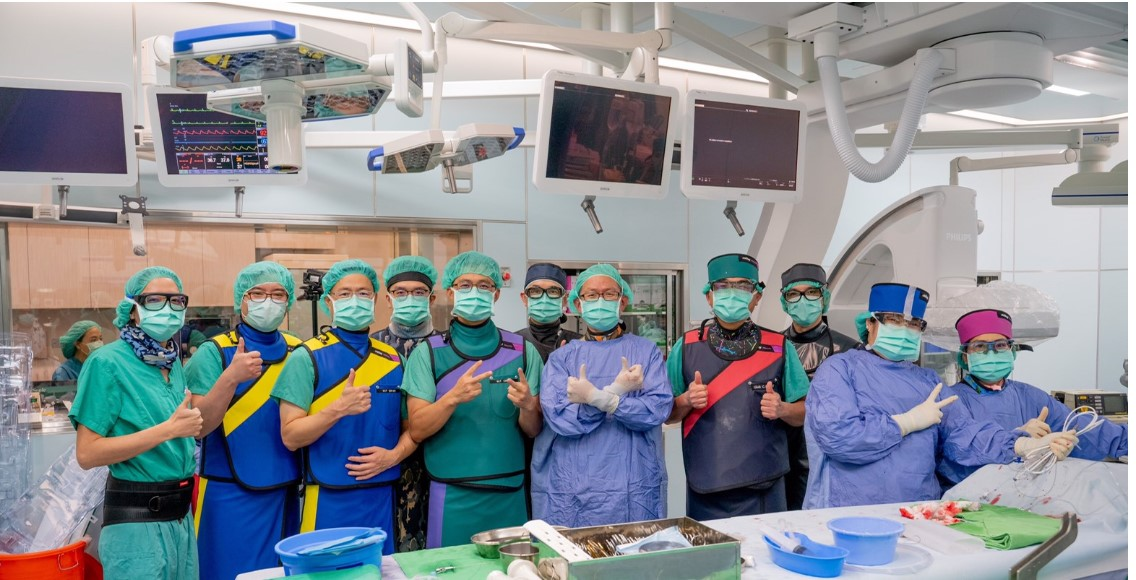
\includegraphics[width=\linewidth]{11001_TMWH_hybrideOT.jpg}
\end{tikzfigure}
}

\block{TMU Main Campus}{%
\begin{tikzfigure}[]
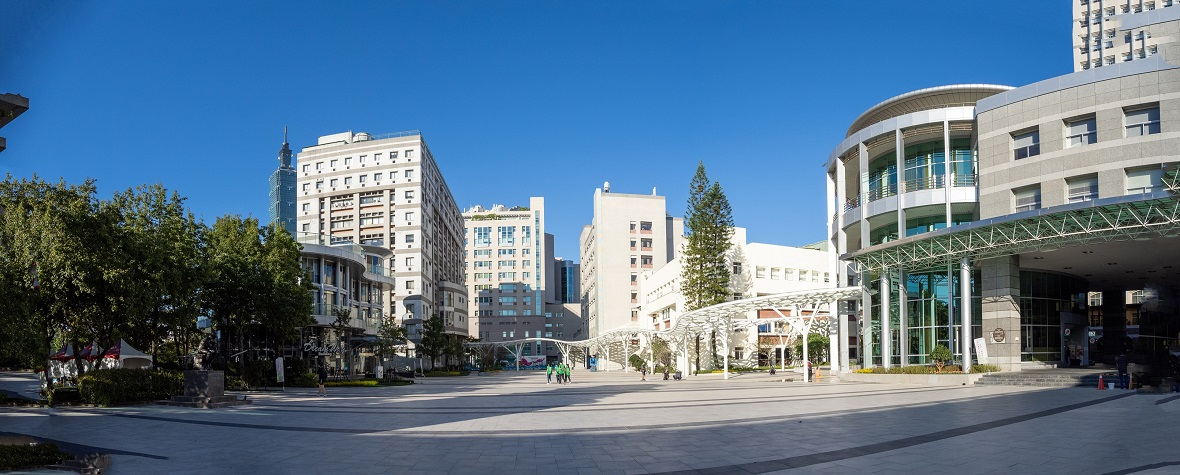
\includegraphics[width=\linewidth]{TMU_4283326b11cfc41667f8cf91f5caaa21.jpg}
\end{tikzfigure}
}


\block{TMU People}{%

\begin{minipage}{0.45\linewidth}
  \centering
\begin{tikzfigure}[]
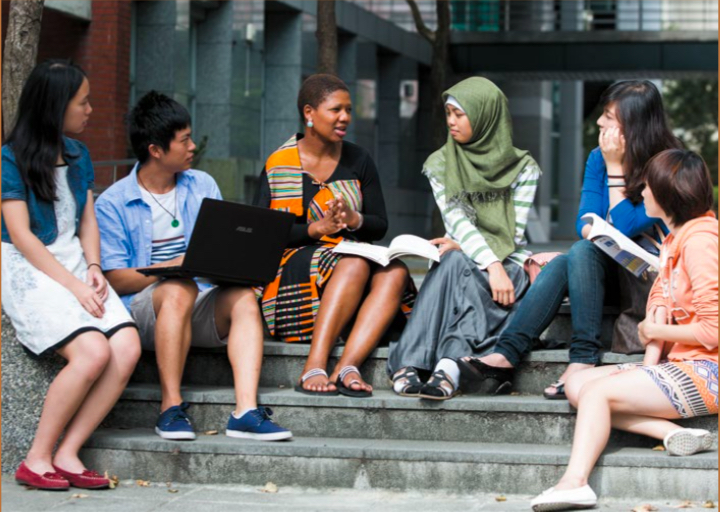
\includegraphics[width=\linewidth]{TMU_students.jpg}
\end{tikzfigure}

\end{minipage}\hfill
\begin{minipage}{0.45\linewidth}
  \centering
\begin{tikzfigure}[]
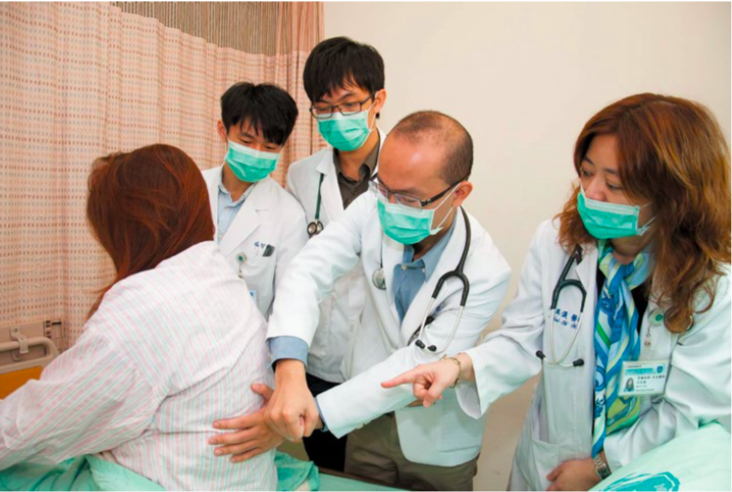
\includegraphics[width=\linewidth]{TMUH_pe.jpg}
\end{tikzfigure}
\end{minipage}

} % end of block

\block{Join TMU}{%

\begin{minipage}{0.3\linewidth}
  \centering
    \begin{tikzfigure}[TMU Intro]
    
\includegraphics[width=0.4\linewidth]{qrcode.66164813.jpg}
%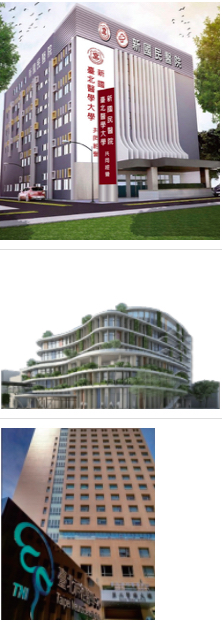
\includegraphics[width=0.5\linewidth]{TMU456.jpg}
    \end{tikzfigure}
\end{minipage}\hfill
\begin{minipage}{0.3\linewidth}
  \centering
\begin{tikzfigure}[]
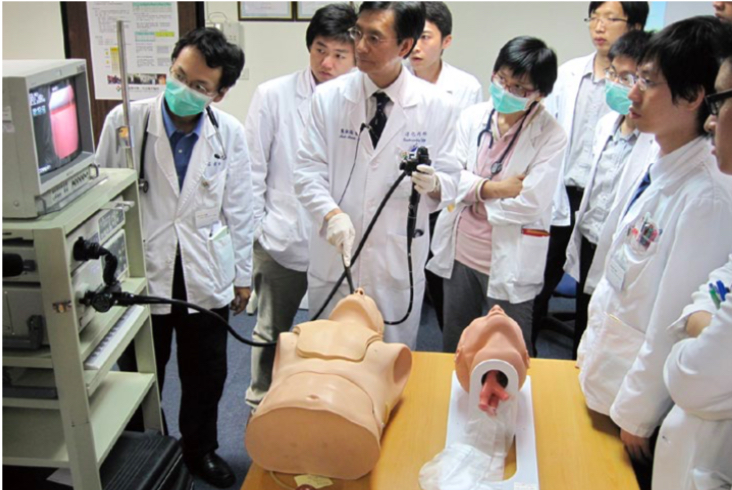
\includegraphics[width=\linewidth]{TMWH_scope.jpg}
\end{tikzfigure}  
\end{minipage}\hfill
\begin{minipage}{0.3\linewidth}
  \centering
\begin{tikzfigure}[International Scholar]

\includegraphics[width=0.5\linewidth]{TMU_QR_sholar.png}
\end{tikzfigure}
\end{minipage}

(* photos courtesy of Public Relation \& Publishing Section, TMU Secretariat)
} % end of block
\end{document}